\documentclass[10pt]{beamer}
\usepackage[utf8]{inputenc}
\usepackage[T1]{fontenc}
\usepackage{graphicx}
\usepackage[numbers]{natbib}
\usepackage{tikz}
\usepackage{amssymb, amsmath, amsfonts}

\colorlet{mybasecolor}[rgb]{blue!50!teal}

\colorlet{mydarkestcolor}[rgb]{mybasecolor!20!black}
\colorlet{mydarkercolor}[rgb]{mybasecolor!40!black}
\colorlet{mydarkcolor}[rgb]{mybasecolor!60!black}
\colorlet{mynormalcolor}[rgb]{mybasecolor!90!black}
\colorlet{mybacklightcolor}[rgb]{mybasecolor!30!white}
\colorlet{mylightcolor}[rgb]{mybasecolor!10!white}

\colorlet{mysidebarcolor}[rgb]{mydarkcolor}
\colorlet{mylogobg}[rgb]{mylightcolor}
\colorlet{mylogofg}[rgb]{mydarkestcolor}
\colorlet{mysidebarauthor}[rgb]{mylightcolor}
\colorlet{mysidebartitle}[rgb]{mylightcolor}
\colorlet{mysidebarsecfg}[rgb]{mydarkestcolor}
\colorlet{mysidebarsecbg}[rgb]{mylightcolor}
\colorlet{mysidebarsubsecfg}[rgb]{mydarkestcolor}
\colorlet{mysidebarsubsecbg}[rgb]{mylightcolor}
\colorlet{myframetitlefg}[rgb]{mylightcolor}
\colorlet{myframetitlebg}[rgb]{mydarkcolor}
\colorlet{myitemcolor}[rgb]{mynormalcolor}
\colorlet{myfontcolor}[rgb]{mydarkestcolor}
\colorlet{mytitlefg}[rgb]{mylightcolor}
\colorlet{mytitlebg}[rgb]{mydarkcolor}
\colorlet{myauthorfg}[rgb]{mylightcolor}
\colorlet{myauthorbg}[rgb]{mydarkcolor}

\useinnertheme{rounded}
\setbeamercolor{structure}{fg = myitemcolor}
\useoutertheme{infolines}

\setbeamercolor{mybox}{bg=mydarkcolor, fg=mylightcolor}
\setbeamercolor{palette primary}  {bg=mydarkestcolor,fg=mylightcolor}
\setbeamercolor{palette secondary}{bg=mydarkcolor,fg=mylightcolor}
\setbeamercolor{palette tertiary} {bg=mydarkercolor,fg=mylightcolor}
\setbeamercolor{palette fourth}   {bg=mydarkcolor,fg=mylightcolor}
\setbeamercolor{title}{bg = mytitlebg,fg = mytitlefg}
\setbeamerfont{title}{series = \bf}
\usefonttheme[onlymath]{serif}

\linespread{1.3}

\newcommand{\mytitle}{
Perfil de Desempenho \\ Rápida Introdução}
\newcommand{\myauthor}{
Abel Soares Siqueira}

\title{\mytitle}
\author{\myauthor}
\date{ }

\newcommand{\myframe}[1]{
\begin{frame}
 %\frametitle{\insertsection \qquad {\small \insertsubsection}}

{#1}

\end{frame}}
\newcommand{\myframetop}[1]{
\begin{frame}[t]
 %\frametitle{\insertsection \qquad {\small \insertsubsection}}

{#1}

\end{frame}}
\newcommand{\ctr}[1]{\begin{center}{\bf #1}\vspace{0.5 cm}\end{center}}

\begin{document}

\myframe{
  \maketitle
}

\myframe{
  Comparação de um conjunto $\mathcal{S}$ de algoritmos usando um conjunto
  $\mathcal{P}$ de problemas.
  \pause

  \ctr{ $t_{p,s} = $ medida de desempenho do algoritmo $s$ para resolver o
    problema $p$}
    \pause
  
  $$ \mbox{medidas} = \left\{ 
    \begin{array}{l} \pause
      \mbox{tempo} \\ \pause
      \mbox{avaliações de função} \\ \pause
      \mbox{?}
    \end{array} \right.$$
  \pause

  $$ \mbox{Falha} \Longrightarrow t_{p,s} = \infty $$
}

\myframe{
  \ctr{ Razão de performance }
  $$r_{p,s} = \dfrac{t_{p,s}}{\min\{t_{p,s}:s\in\mathcal{S}\}}$$
  \pause

  $$ r_{p,s} \geq 1 $$
  \pause
  $$ r_M = \max\{ r_{p,s} : r_{p,s} < \infty \} $$
  \pause
  Se o algoritmo $s$ converge para o problema $p$, então
  $r_{p,s} \leq r_M$.
}

\myframe{
  \ctr{ Curva de performance }
  $$ \rho_s(\tau) = \frac{1}{ |\mathcal{P}| }
  |\{p \in \mathcal{P} : r_{p,s} \leq \tau \}|. $$
  \pause
  $\rho_s(\tau)$ é a porcentagem de problemas que o algoritmo $s$ resolve com
  até o tempo escalado $\tau$.
}

\myframe{
  Note que a interpretação para um $\tau$ qualquer não é trivial, mas para dois
  valores de $\tau$, podemos retirar conclusões definitivas.
  \pause

  \vspace{1.0cm}
  \begin{center}
  \begin{minipage}{0.43\textwidth}
    \ctr{Eficiência $\tau = 1$}
    Em que porcentagem de problemas o algoritmo $s$ é mais rápido que os outros.
  \end{minipage}
  \hspace{0.1\textwidth}
  \begin{minipage}{0.43\textwidth}
    \ctr{Robustez $\tau = r_M$}
    Que porcentagem de problemas o algoritmo $s$ resolve.
  \end{minipage}
  \end{center}
}

\myframetop{
  \ctr{Exemplo}
  \begin{center}
    Tempo para o algoritmo ser resolvido (em $s$).
  \begin{tabular}{|c|c|c|c|} \hline
    {\bf Problema} &
    {Algoritmo 1} &
    {Algoritmo 2} &
    {Algoritmo 3} \\ \hline
    1 &  0.01 & 0.02 &  0.09 \\ \hline
    2 &  0.15 & 0.04 &   -  \\ \hline
    3 &  1.00 & 1.00 &  0.5 \\ \hline
    4 & 12.00 & 9.50 &  9.0 \\ \hline
    5 &    -  &    - & 59.0 \\ \hline
  \end{tabular}
  \end{center}
}

\myframetop{
  \ctr{Exemplo}
  \begin{center}
    Razão de performance ($r_{p,s}$).
  \begin{tabular}{|c|c|c|c|} \hline
    {\bf Problema} &
    {Algoritmo 1} &
    {Algoritmo 2} &
    {Algoritmo 3} \\ \hline
    1 &     1.00 &     2.00 &     9.00 \\ \hline
    2 &     3.75 &     1.00 & $\infty$ \\ \hline
    3 &     2.00 &     2.00 &     1.00 \\ \hline
    4 &     1.33 &     1.06 &     1.00 \\ \hline
    5 & $\infty$ & $\infty$ &     1.00 \\ \hline
  \end{tabular}
  $$ r_M = 9. $$
  \end{center}
}

\myframetop{
  \ctr{Exemplo}
  \begin{center}
  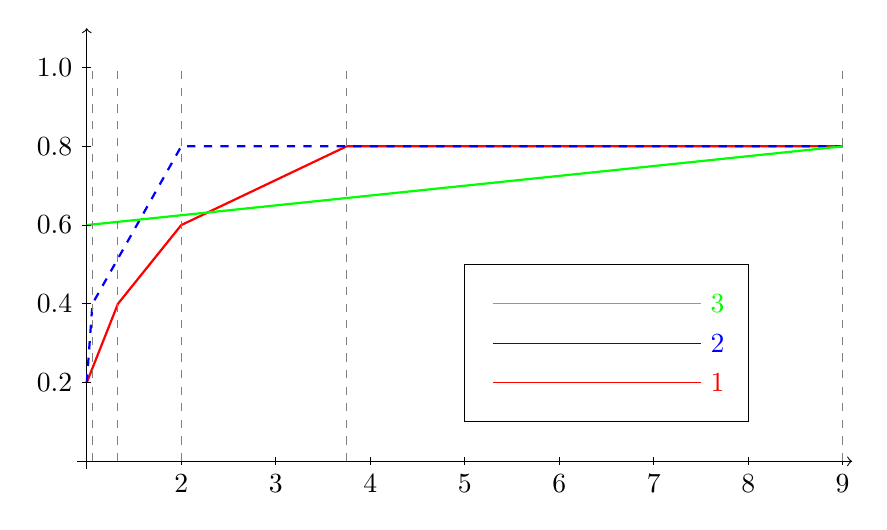
\begin{tikzpicture}[yscale=5,xscale=1.2]
    \draw[->] (0.9,0) -- (9.1,0);
    \draw[->] (1,-0.02) -- (1,1.1);
    \draw[thick,red] 
      (1,1/5) -- 
      (1.33,2/5) --
      (2,3/5) --
      (3.75,4/5) --
      (9.00,4/5);
    \draw[dashed,thick,blue]
      (1,1/5) -- 
      (1.06,2/5) -- 
      (2,4/5) --
      (9,4/5);
    \draw[thick,green]
      (1,3/5) --
      (9,4/5);
    \foreach \x in {2,3,...,9} {
      \draw (\x,0.01) -- (\x,-0.01) node[below]{\x};
    }
    \foreach \x in {1.06, 1.33, 2, 3.75, 9} {
      \only<2>{\draw[dashed,thin,gray] (\x,0) -- (\x,1);}
    }
    \foreach \y in {0.2,0.4,0.6,0.8,1.0} {
      \draw (1.05,\y) -- (0.95,\y) node[left]{\y};
    }
    \draw (5,0.1) rectangle (8,0.5);
    \draw[red]  (5.3,0.2) -- (7.5,0.2) node[right]{1};
    \draw[blue] (5.3,0.3) -- (7.5,0.3) node[right]{2};
    \draw[green](5.3,0.4) -- (7.5,0.4) node[right]{3};
  \end{tikzpicture}
  \end{center}
}

\myframe{
  {\bf Não} necessariamente 
  $$\sum_{s=1}^{|\mathcal{S}|}\rho_s(1) \leq 1$$
  pois os algoritmos podem empatar para alguns problemas.
  \pause

  O que eu uso pra gerar?
  \begin{itemize}
    \item<2-> Para poucos problemas, talvez usar o matlab introduzindo os dados a
      mão é suficiente.
    \item<3-> Para muitos problemas, é melhor criar algum script em Bash,
      Python, ou o que preferir.
    \item<4-> Faça com que seu algoritmo imprima os resultados de uma maneira
      fácil de ser lida por uma máquina.
  \end{itemize}
}

\myframe{
  Um exemplo mais avançado. Implementamos
  \begin{itemize}
    \item<2-> Método de Busca Direcional (Direct Search)
    \item<3-> Método Nelder-Mead (Nelmer-Mead)
  \end{itemize}
}

\myframe{
  \pgfdeclareimage[width=0.95\textwidth]{profile}{tests/profile}
  \pgfdeclareimage[width=0.95\textwidth]{profilelog}{tests/profile_log}
  \pgfuseimage{profile}<1>
  \pgfuseimage{profilelog}<2>
}

\end{document}
